% Asset ID: FA22GeneratingFunctionsTikZ-002
% Unit: FA22 – Further A2 2 Applied Mathematics
% Topic code: FA22-GENFUNC
% Topic ID: FA22GeneratingFunctions
% Related lesson: FA22_generating_functions_lesson.md
% Source status: Optional enrichment, not confirmed CCEA core
\documentclass[tikz,border=8pt]{standalone}
\usepackage{amsmath}\usepackage{xcolor}\usetikzlibrary{arrows.meta,positioning,calc,matrix}
\definecolor{Canvas}{HTML}{FAF9F6}\definecolor{Ivory}{HTML}{FFFFF0}\definecolor{Line}{HTML}{E5E5EA}\definecolor{Gold}{HTML}{C5A059}\definecolor{SoftPink}{HTML}{FBEFEF}\definecolor{Text}{HTML}{2C2C2E}
\begin{document}
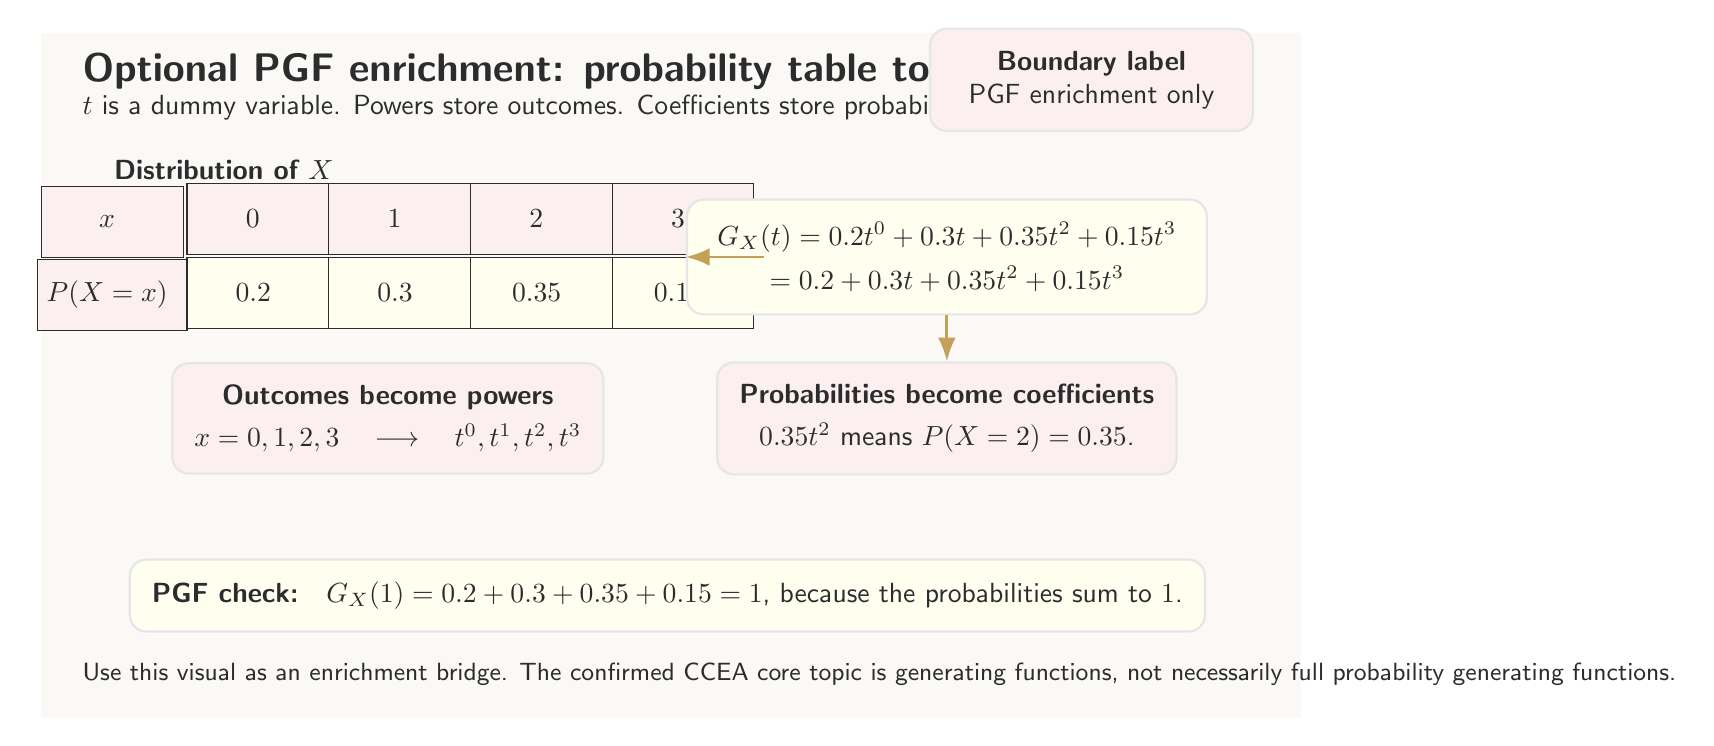
\begin{tikzpicture}[font=\sffamily,text=Text,cell/.style={draw=Text,fill=Ivory,minimum width=1.8cm,minimum height=0.9cm,align=center},header/.style={draw=Text,fill=SoftPink,minimum width=1.8cm,minimum height=0.9cm,align=center,font=\sffamily\bfseries},box/.style={draw=Line,fill=Ivory,rounded corners=6pt,line width=0.8pt,align=center,inner sep=8pt},accentbox/.style={draw=Line,fill=SoftPink,rounded corners=6pt,line width=0.8pt,align=center,inner sep=8pt},arrow/.style={-{Latex[length=3mm]},line width=1pt,draw=Gold}]
\fill[Canvas] (-0.8,-3.1) rectangle (15.2,5.6);
\node[anchor=west,font=\sffamily\bfseries\Large] at (-0.4,5.1){Optional PGF enrichment: probability table to polynomial};
\node[anchor=west,font=\sffamily\normalsize] at (-0.4,4.65){\(t\) is a dummy variable. Powers store outcomes. Coefficients store probabilities.};
\node[accentbox,anchor=east,minimum width=4.1cm] at (14.6,5.0){\textbf{Boundary label}\\PGF enrichment only};
\node[anchor=west,font=\sffamily\bfseries] at (0.0,3.85){Distribution of \(X\)};
\matrix (table) [matrix of nodes,nodes in empty cells,row sep=-\pgflinewidth,column sep=-\pgflinewidth,ampersand replacement=\&,column 1/.style={nodes={header}},row 1/.style={nodes={header}},nodes={cell}] at (3.7,2.75){\(x\) \& \(0\) \& \(1\) \& \(2\) \& \(3\) \\ \(P(X=x)\) \& \(0.2\) \& \(0.3\) \& \(0.35\) \& \(0.15\) \\};
\node[box,minimum width=6.6cm,minimum height=1.45cm] (pgf) at (10.7,2.75){\(\displaystyle G_X(t)=0.2t^0+0.3t+0.35t^2+0.15t^3\)\\[4pt]\(\displaystyle =0.2+0.3t+0.35t^2+0.15t^3\)};
\draw[arrow] (table.east) -- (pgf.west);
\node[accentbox,minimum width=5.4cm] (powers) at (3.6,0.7){\textbf{Outcomes become powers}\\[3pt]\(x=0,1,2,3\quad \longrightarrow \quad t^0,t^1,t^2,t^3\)};
\node[accentbox,minimum width=5.4cm] (coeffs) at (10.7,0.7){\textbf{Probabilities become coefficients}\\[3pt]\(0.35t^2\) means \(P(X=2)=0.35\).};
\draw[arrow] (pgf.south) -- (coeffs.north);
\node[box,minimum width=12.4cm] at (7.15,-1.55){\textbf{PGF check:}\quad \(\displaystyle G_X(1)=0.2+0.3+0.35+0.15=1\), because the probabilities sum to \(1\).};
\node[anchor=west,font=\sffamily\small] at (-0.4,-2.55){Use this visual as an enrichment bridge. The confirmed CCEA core topic is generating functions, not necessarily full probability generating functions.};
\end{tikzpicture}
\end{document}
